% Topic 2.1: Digital Payments -- How Money Actually Moves
% Digital Finance Course - Problem-driven BSc-level module
% Rewritten: No specific numbers, company stats, or dollar amounts
\documentclass[11pt,aspectratio=169]{beamer}
\usetheme{Madrid}

% ======================= PACKAGES =======================
\usepackage{graphicx}
\usepackage{booktabs}
\usepackage{adjustbox}
\usepackage{multicol}
\usepackage{amsmath}
\usepackage{amssymb}
\usepackage{tikz}
\usetikzlibrary{arrows,shapes,positioning,shadows,trees}
\usepackage{listings}
\usepackage{xcolor}

% ======================= COLOR DEFINITIONS =======================
% Primary color scheme: Blue/Teal for Digital Finance
\definecolor{dfblue}{RGB}{0,102,204}
\definecolor{dfteal}{RGB}{0,153,153}
\definecolor{dfcyan}{RGB}{51,187,204}
\definecolor{dflightblue}{RGB}{153,204,255}
\definecolor{dflightblue2}{RGB}{173,214,255}
\definecolor{dflightblue3}{RGB}{193,224,255}
\definecolor{dflightblue4}{RGB}{213,234,255}

% Accent colors for finance applications
\definecolor{dfgreen}{RGB}{44, 160, 44}
\definecolor{dfred}{RGB}{214, 39, 40}
\definecolor{dforange}{RGB}{255, 127, 14}
\definecolor{dfgray}{RGB}{127, 127, 127}

% Utility colors
\definecolor{lightgray}{RGB}{240, 240, 240}
\definecolor{midgray}{RGB}{180, 180, 180}
\definecolor{codebg}{RGB}{245, 245, 245}

% ======================= THEME CUSTOMIZATION =======================
% Apply Digital Finance color scheme to Madrid theme
\setbeamercolor{palette primary}{bg=dflightblue3,fg=dfblue}
\setbeamercolor{palette secondary}{bg=dflightblue2,fg=dfblue}
\setbeamercolor{palette tertiary}{bg=dfteal,fg=white}
\setbeamercolor{palette quaternary}{bg=dfblue,fg=white}

\setbeamercolor{structure}{fg=dfblue}
\setbeamercolor{section in toc}{fg=dfblue}
\setbeamercolor{subsection in toc}{fg=dfteal}
\setbeamercolor{title}{fg=dfblue}
\setbeamercolor{frametitle}{fg=dfblue,bg=dflightblue3}
\setbeamercolor{block title}{bg=dflightblue2,fg=dfblue}
\setbeamercolor{block body}{bg=dflightblue4,fg=black}

% Remove navigation symbols for cleaner look
\setbeamertemplate{navigation symbols}{}

% Clean itemize/enumerate
\setbeamertemplate{itemize items}[circle]
\setbeamertemplate{enumerate items}[default]

% Margins for readability
\setbeamersize{text margin left=8mm,text margin right=8mm}

% ======================= LISTINGS CONFIGURATION =======================
% Python code style
\lstdefinestyle{pythonstyle}{
    language=Python,
    basicstyle=\ttfamily\footnotesize,
    keywordstyle=\color{dfblue}\bfseries,
    stringstyle=\color{dforange},
    commentstyle=\color{dfgray}\itshape,
    numberstyle=\tiny\color{dfgray},
    numbers=left,
    numbersep=5pt,
    backgroundcolor=\color{codebg},
    showspaces=false,
    showstringspaces=false,
    showtabs=false,
    frame=single,
    rulecolor=\color{midgray},
    tabsize=4,
    captionpos=b,
    breaklines=true,
    breakatwhitespace=false,
    escapeinside={(*@}{@*)},
    xleftmargin=10pt,
    xrightmargin=10pt
}

% Solidity code style
\lstdefinestyle{soliditystyle}{
    language=Java, % closest approximation
    basicstyle=\ttfamily\footnotesize,
    keywordstyle=\color{dfteal}\bfseries,
    stringstyle=\color{dforange},
    commentstyle=\color{dfgray}\itshape,
    numberstyle=\tiny\color{dfgray},
    numbers=left,
    numbersep=5pt,
    backgroundcolor=\color{codebg},
    showspaces=false,
    showstringspaces=false,
    showtabs=false,
    frame=single,
    rulecolor=\color{midgray},
    tabsize=2,
    captionpos=b,
    breaklines=true,
    breakatwhitespace=false,
    escapeinside={(*@}{@*)},
    xleftmargin=10pt,
    xrightmargin=10pt,
    morekeywords={pragma, contract, function, returns, public, private, view, pure, payable, address, uint256, mapping, event, modifier}
}

% Inline code command
\newcommand{\code}[1]{\texttt{\color{dfblue}#1}}

% ======================= CUSTOM COMMANDS =======================
% Bottom annotation (Madrid-style)
\newcommand{\bottomnote}[1]{%
\vfill
\vspace{-2mm}
\textcolor{dflightblue2}{\rule{\textwidth}{0.4pt}}
\vspace{1mm}
\footnotesize
\textbf{#1}
}

% Compact list spacing
\newcommand{\compactlist}{%
\setlength{\itemsep}{0pt}%
\setlength{\parskip}{0pt}%
\setlength{\parsep}{0pt}%
}

% Chart placeholder
\newcommand{\chartplaceholder}[2][5cm]{%
\begin{center}
\begin{adjustbox}{max width=0.95\textwidth, max height=#1}
\framebox[\textwidth][c]{%
\rule{0pt}{#1}%
\textcolor{midgray}{[#2]}%
}
\end{adjustbox}
\end{center}
}

% ======================= FINANCE NOTATION MACROS =======================
% Probability and statistics
\newcommand{\E}{\mathbb{E}} % Expected value
\newcommand{\Var}{\mathrm{Var}} % Variance
\newcommand{\Cov}{\mathrm{Cov}} % Covariance
\newcommand{\Prob}{\mathbb{P}} % Probability

% Distributions
\newcommand{\Normal}{\mathcal{N}} % Normal distribution
\newcommand{\Uniform}{\mathcal{U}} % Uniform distribution

% Returns and prices
\newcommand{\Ret}{R} % Return
\newcommand{\LogRet}{r} % Log return
\newcommand{\Price}{S} % Price/Stock price
\newcommand{\Strike}{K} % Strike price

% Options and derivatives
\newcommand{\CallPrice}{C} % Call option price
\newcommand{\PutPrice}{P} % Put option price
\newcommand{\Greeks}[1]{\mathit{#1}} % Greek letters

% Risk measures
\newcommand{\VaR}{\mathrm{VaR}} % Value at Risk
\newcommand{\CVaR}{\mathrm{CVaR}} % Conditional VaR
\newcommand{\Sharpe}{\mathrm{SR}} % Sharpe Ratio

% Time series
\newcommand{\AR}{\mathrm{AR}} % Autoregressive
\newcommand{\MA}{\mathrm{MA}} % Moving average
\newcommand{\GARCH}{\mathrm{GARCH}} % GARCH

% Blockchain/Crypto
\newcommand{\Hash}{\mathrm{Hash}} % Hash function
\newcommand{\Block}{\mathcal{B}} % Block
\newcommand{\Chain}{\mathcal{C}} % Chain

% Real numbers, integers
\newcommand{\R}{\mathbb{R}}
\newcommand{\Z}{\mathbb{Z}}
\newcommand{\N}{\mathbb{N}}

% ======================= TIKZ STYLES =======================
% Styles for finance-related diagrams
\tikzstyle{process} = [rectangle, minimum width=3cm, minimum height=1cm, text centered, draw=dfblue, fill=dflightblue4, thick]
\tikzstyle{decision} = [diamond, minimum width=3cm, minimum height=1cm, text centered, draw=dfteal, fill=dflightblue4, thick]
\tikzstyle{arrow} = [thick,->,>=stealth,color=dfblue]
\tikzstyle{blockchain} = [rectangle, rounded corners, minimum width=2.5cm, minimum height=1cm, text centered, draw=dfteal, fill=dflightblue3, thick]
\tikzstyle{transaction} = [circle, minimum size=0.8cm, text centered, draw=dforange, fill=dflightblue4, thick]

% ======================= FOOTER TEMPLATE =======================
\setbeamertemplate{footline}{
    \hbox{\begin{beamercolorbox}[wd=\paperwidth,ht=2.5ex,dp=1ex,leftskip=.5em,rightskip=.5em]{author in head/foot}
    \tiny
    \textbf{Digital Finance} \hfill
    Joerg Osterrieder \hfill
    \insertdate \hfill
    Page \insertframenumber{} / \inserttotalframenumber
    \end{beamercolorbox}}
}

% ======================= SECTION DIVIDER TEMPLATE =======================
\AtBeginSection[]{
\begin{frame}[plain]
\vfill
\centering
\begin{beamercolorbox}[sep=12pt,center]{title}
\usebeamerfont{title}\LARGE\insertsection\par
\end{beamercolorbox}
\vfill
\end{frame}
}


\title[T2.1: Digital Payments]{Topic 2.1: Digital Payments}
\subtitle{How Money Actually Moves}
\author{Joerg Osterrieder}
\institute{Digital Finance}
\date{Digital Finance}

\begin{document}

% ==================== SLIDE 1: TITLE ====================
\begin{frame}[plain]
\titlepage
\end{frame}

% ==================== SLIDE 2: LEARNING OBJECTIVES ====================
\begin{frame}{Learning Objectives}
\begin{block}{By the end of this topic, you will be able to:}
\begin{enumerate}
\item \textbf{Explain} the four-layer payment stack and identify each layer's function
\item \textbf{Trace} a card payment from initiation to settlement using the four-party model
\item \textbf{Compare} payment methods by speed, cost, and consumer protection trade-offs
\item \textbf{Analyze} the conceptual economics of interchange and explain why payment fees exist
\item \textbf{Evaluate} how FinTech innovations challenge traditional payment infrastructure
\item \textbf{Apply} payment analysis techniques to transaction data (NB02)
\end{enumerate}
\end{block}

\vspace{3mm}
\textbf{Key Competency}: Trace a digital payment from initiation to settlement and identify where value is captured at each layer.
\end{frame}

% ==================== SLIDE 3: PREREQUISITES ====================
\begin{frame}{Prerequisites: What is a Payment?}
\begin{columns}[T]
\begin{column}{0.5\textwidth}
\textbf{Definition:}\\
A \textcolor{dfblue}{\textbf{payment}} is the transfer of value from one party (payer) to another (payee) in exchange for goods, services, or to fulfill an obligation.

\vspace{4mm}
\textbf{Three Essential Components:}
\begin{enumerate}
\item \textbf{Instruction}: The order to transfer funds
\item \textbf{Clearing}: Verification and reconciliation of the transaction between parties
\item \textbf{Settlement}: The final, irrevocable transfer of money
\end{enumerate}
\end{column}
\begin{column}{0.5\textwidth}
\begin{alertblock}{The Hidden Complexity}
What seems simple is actually complex. When you tap your card at a coffee shop, what actually happens in the next few seconds --- and the next few days?
\end{alertblock}

\vspace{3mm}
\begin{block}{Key Terms}
\begin{itemize}
\item \textbf{Payer}: Person or entity sending money
\item \textbf{Payee}: Person or entity receiving money
\item \textbf{Settlement}: When funds actually move
\item \textbf{Float}: The gap between approval and settlement
\end{itemize}
\end{block}
\end{column}
\end{columns}

\vspace{2mm}
\begin{block}{The Insight}
The gap between ``approved'' and ``money moved'' is where enormous value is created and captured.
\end{block}
\end{frame}

% ==================== SLIDE 4: THE PAYMENT STACK ====================
\begin{frame}{The Hidden Journey of a Payment}
\begin{alertblock}{The Problem}
Why does a simple coffee purchase involve so many parties?
\end{alertblock}

\vspace{2mm}
\begin{center}
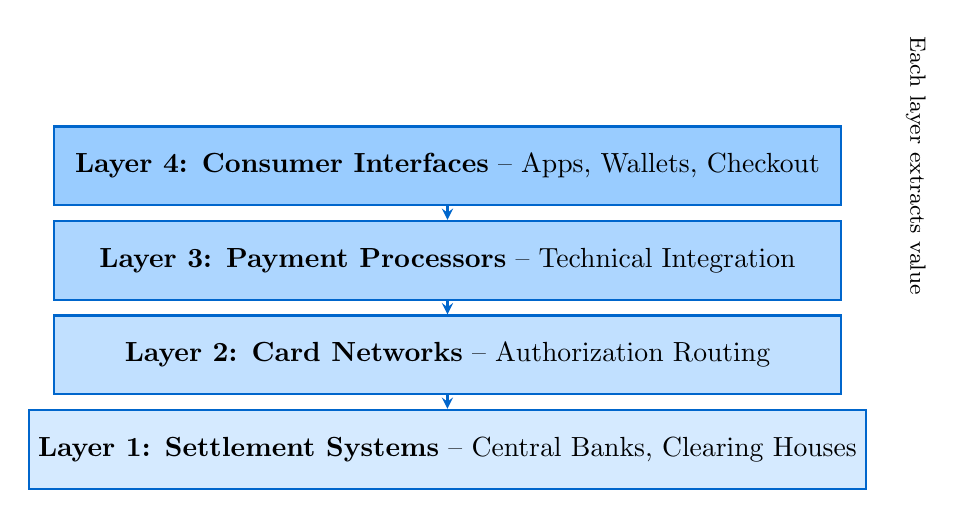
\begin{tikzpicture}[node distance=1.2cm]
% Layer boxes - generic labels, no company names
\node (l4) [process, minimum width=10cm, fill=dflightblue] {\textbf{Layer 4: Consumer Interfaces} -- Apps, Wallets, Checkout};
\node (l3) [process, minimum width=10cm, below of=l4, fill=dflightblue2] {\textbf{Layer 3: Payment Processors} -- Technical Integration};
\node (l2) [process, minimum width=10cm, below of=l3, fill=dflightblue3] {\textbf{Layer 2: Card Networks} -- Authorization Routing};
\node (l1) [process, minimum width=10cm, below of=l2, fill=dflightblue4] {\textbf{Layer 1: Settlement Systems} -- Central Banks, Clearing Houses};

% Arrows
\draw[arrow] (l4) -- (l3);
\draw[arrow] (l3) -- (l2);
\draw[arrow] (l2) -- (l1);

% Side label
\node[right of=l4, xshift=4.5cm, rotate=-90, anchor=south, font=\footnotesize] {Each layer extracts value};
\end{tikzpicture}
\end{center}
\end{frame}

% ---- The Hidden Journey of a Payment (cont.) ----
\begin{frame}{The Hidden Journey of a Payment (cont.)}
\begin{block}{The Insight}
Each layer in the payment stack captures a portion of every transaction. Understanding the stack reveals who profits from your purchase --- and where disruption is possible.
\end{block}
\end{frame}

% ==================== SLIDE 5: LAYER 1 - SETTLEMENT SYSTEMS ====================
\begin{frame}{Layer 1: Settlement Systems}
\begin{alertblock}{The Problem}
How does money \textit{actually} move between banks?
\end{alertblock}

\vspace{2mm}
\begin{columns}[T]
\begin{column}{0.5\textwidth}
\textbf{The Concept:}
\begin{itemize}\compactlist
\item \textbf{Settlement} = the final, irrevocable transfer of money between banks
\item Operated by central banks or banking consortia
\item The foundation on which all other payment layers are built
\item Different systems exist for domestic vs.\ international transfers
\end{itemize}

\vspace{2mm}
\textbf{Authorization vs.\ Settlement:}
\begin{itemize}\compactlist
\item \textbf{Authorization}: ``Yes, this payment is approved'' --- happens in seconds (like making a reservation)
\item \textbf{Settlement}: ``Money has actually moved'' --- can take days (like completing the transaction)
\end{itemize}
\end{column}
\begin{column}{0.5\textwidth}
\begin{block}{The Float}
You can spend money in seconds that takes days to actually move. This gap is called \textbf{float}\footnotemark --- and it creates both risk and opportunity.

\vspace{1mm}
\textit{During the float period:}
\begin{itemize}\compactlist
\item The merchant does not yet have the funds
\item The payer's bank has reserved but not released the money
\item Intermediaries may earn interest on funds in transit
\end{itemize}
\end{block}
\footnotetext{Float --- the time money is ``in transit'' between accounts, during which neither party can fully use it.}
\end{column}
\end{columns}
\end{frame}

% ---- Layer 1: Settlement Systems (cont.) ----
\begin{frame}{Layer 1: Settlement Systems (cont.)}
\begin{block}{The Insight}
The delay between ``approved'' and ``settled'' is not a bug --- it is where significant economic value is created.
\end{block}
\end{frame}

% ==================== SLIDE 6: LAYER 2 - CARD NETWORKS ====================
\begin{frame}{Layer 2: Card Networks}
\begin{alertblock}{The Problem}
How does your card work at a store on the other side of the world?
\end{alertblock}

\vspace{1mm}
\begin{columns}[T]
\begin{column}{0.5\textwidth}
\textbf{The Concept:}
\begin{itemize}\compactlist
\item Card networks connect \textbf{issuing banks}\footnotemark[1] to \textbf{acquiring banks}\footnotemark[2]
\item They route authorization requests across borders
\item They set rules, standards, and manage fraud liability
\item The largest networks operate globally, accepted nearly everywhere
\end{itemize}
\footnotetext[1]{Issuing bank --- your bank that issued your card.}
\footnotetext[2]{Acquiring bank --- the merchant's bank that receives payments on their behalf.}
\end{column}
\begin{column}{0.5\textwidth}
\begin{block}{Network Effects Create Dominance}
\begin{center}
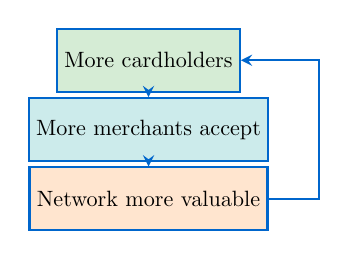
\begin{tikzpicture}[node distance=1.1cm, scale=0.8, transform shape]
\node (more) [process, fill=dfgreen!20, minimum width=2.8cm] {More cardholders};
\node (accept) [process, fill=dfteal!20, below of=more, minimum width=2.8cm] {More merchants accept};
\node (value) [process, fill=dforange!20, below of=accept, minimum width=2.8cm] {Network more valuable};
\draw[arrow] (more) -- (accept);
\draw[arrow] (accept) -- (value);
\draw[arrow] (value.east) -- ++(0.8,0) |- (more.east);
\end{tikzpicture}
\end{center}
\textit{Merchants accept what consumers carry. Consumers carry what merchants accept.}
\end{block}
\end{column}
\end{columns}

\vspace{1mm}
\begin{block}{The Insight}
Network effects create a self-reinforcing cycle --- once a card network reaches critical mass, it becomes extremely difficult to displace.
\end{block}
\end{frame}

% ==================== SLIDE 7: LAYER 3 - PAYMENT PROCESSORS ====================
\begin{frame}{Layer 3: Payment Processors}
\begin{alertblock}{The Problem}
Why can't merchants just connect directly to card networks?
\end{alertblock}

\vspace{2mm}
\begin{columns}[T]
\begin{column}{0.5\textwidth}
\textbf{The Concept:}
\begin{itemize}\compactlist
\item Connecting directly to networks requires complex technical integration and regulatory compliance
\item \textbf{Payment processors} handle this complexity on behalf of merchants
\item They provide fraud detection, developer tools (APIs), and multi-network routing
\item They charge a small markup on each transaction for this service
\end{itemize}
\end{column}
\begin{column}{0.5\textwidth}
\begin{block}{Before vs.\ After Processors}
\textbf{Without processors:}
\begin{itemize}\compactlist
\item Custom bank integration
\item Months of development
\item Complex compliance requirements
\item Network-by-network negotiation
\end{itemize}

\vspace{1mm}
\textbf{With processors:}
\begin{itemize}\compactlist
\item Simple API integration
\item Fast setup
\item Bundled compliance and fraud protection
\item Multi-network routing in one package
\end{itemize}
\end{block}
\end{column}
\end{columns}
\end{frame}

% ---- Layer 3: Payment Processors (cont.) ----
\begin{frame}{Layer 3: Payment Processors (cont.)}
\begin{block}{The Insight}
By simplifying integration, processors unlocked payment innovation for millions of businesses that could never have connected to networks on their own.
\end{block}
\end{frame}

% ==================== SLIDE 8: LAYER 4 - CONSUMER INTERFACES ====================
\begin{frame}{Layer 4: Consumer Interfaces}
\begin{alertblock}{The Problem}
Why is every tech company building a wallet or payment app?
\end{alertblock}

\vspace{2mm}
\begin{columns}[T]
\begin{column}{0.5\textwidth}
\textbf{The Concept:}
\begin{itemize}\compactlist
\item The interface layer is the user-facing payment experience
\item It stores payment credentials securely
\item Types include: mobile wallets, peer-to-peer apps, e-commerce checkout, point-of-sale terminals, bank apps
\end{itemize}

\vspace{2mm}
\textbf{Why Everyone Wants This Layer:}
\begin{itemize}\compactlist
\item Owns the \textbf{customer relationship}
\item Captures \textbf{spending data}
\item Enables \textbf{cross-selling} other products
\item Builds \textbf{brand loyalty}
\end{itemize}
\end{column}
\begin{column}{0.5\textwidth}
\begin{alertblock}{Where Competition Happens}
Most FinTech innovation targets this layer because it is closest to the customer.

\vspace{1mm}
The underlying rails (networks, settlement) remain largely unchanged --- the battle is over who controls the experience on top.
\end{alertblock}

\vspace{1mm}
\begin{exampleblock}{Think About It}
How many different payment apps are on your phone right now? Each one is competing for this layer.
\end{exampleblock}
\end{column}
\end{columns}
\end{frame}

% ---- Layer 4: Consumer Interfaces (cont.) ----
\begin{frame}{Layer 4: Consumer Interfaces (cont.)}
\begin{block}{The Insight}
The real battle in payments is not moving money --- it is \textbf{owning the customer relationship}.
\end{block}
\end{frame}

% ==================== SLIDE 9: THE FOUR-PARTY MODEL ====================
\begin{frame}{The Four-Party Model}
\begin{alertblock}{The Problem}
When you swipe your card, who is involved and what happens?
\end{alertblock}

\vspace{2mm}
\begin{center}
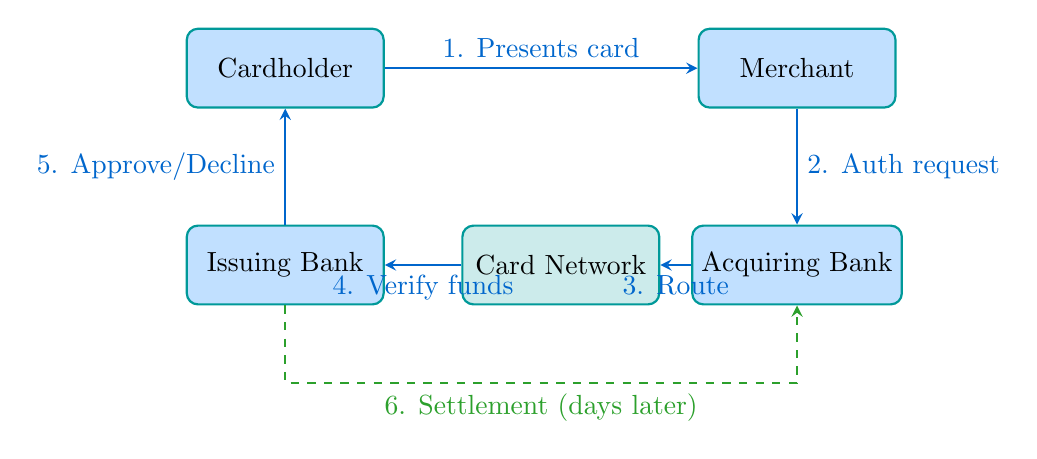
\begin{tikzpicture}[node distance=2.5cm, auto]
% Nodes
\node (cardholder) [blockchain] {Cardholder};
\node (merchant) [blockchain, right of=cardholder, xshift=4cm] {Merchant};
\node (issuer) [blockchain, below of=cardholder] {Issuing Bank};
\node (acquirer) [blockchain, below of=merchant] {Acquiring Bank};
\node (network) [blockchain, below of=cardholder, xshift=3.5cm, fill=dfteal!20] {Card Network};

% Arrows - NO dollar amounts
\draw[arrow] (cardholder) -- node[above] {1. Presents card} (merchant);
\draw[arrow] (merchant) -- node[right] {2. Auth request} (acquirer);
\draw[arrow] (acquirer) -- node[below] {3. Route} (network);
\draw[arrow] (network) -- node[below] {4. Verify funds} (issuer);
\draw[arrow] (issuer) -- node[left] {5. Approve/Decline} (cardholder);
\draw[arrow, dashed, color=dfgreen] (issuer) |- ++(0,-1.5) -| node[below, pos=0.25] {6. Settlement (days later)} (acquirer);
\end{tikzpicture}
\end{center}
\end{frame}

% ---- The Four-Party Model (cont.) ----
\begin{frame}{The Four-Party Model (cont.)}
\begin{block}{The Insight}
Authorization happens in seconds; settlement takes days. The merchant sees ``approved'' almost instantly, but the actual money moves much later in batch processing.
\end{block}
\end{frame}

% ==================== SLIDE 10: WHO PAYS WHOM ====================
\begin{frame}{Who Pays Whom?}
\begin{alertblock}{The Problem}
Who actually pays for the ``free'' card in your wallet?
\end{alertblock}

\vspace{3mm}
\begin{center}
\begin{tabular}{p{2.8cm}p{4.5cm}p{4cm}}
\toprule
\textbf{Party} & \textbf{Role} & \textbf{How They Earn} \\
\midrule
\textbf{Cardholder} & Initiates payment & (Consumer --- pays indirectly through prices) \\
\textbf{Merchant} & Accepts payment & Sells goods/services \\
\textbf{Issuing Bank} & Issues card, bears risk & Receives the largest share of fees \\
\textbf{Acquiring Bank} & Processes for merchant & Keeps a small portion of fees \\
\textbf{Card Network} & Routes transactions & Charges assessment fees \\
\bottomrule
\end{tabular}
\end{center}

\vspace{3mm}
\textbf{The Fee Flow:}
Merchant pays $\rightarrow$ Acquirer passes on $\rightarrow$ Network routes $\rightarrow$ Issuer receives most

\vspace{2mm}
\begin{block}{The Insight}
The \textbf{issuing bank} receives the largest share because it bears the credit and fraud risk. The merchant passes these costs into prices --- so consumers ultimately pay, even if their card is ``free.''
\end{block}
\end{frame}

% ==================== SLIDE 11: THE COST OF CONVENIENCE ====================
\begin{frame}{The Cost of Convenience}
\begin{alertblock}{The Problem}
Why do card payments cost merchants more than a simple bank transfer?
\end{alertblock}

\vspace{2mm}
\begin{columns}[T]
\begin{column}{0.5\textwidth}
\textbf{What Interchange Fees Pay For:}
\begin{itemize}\compactlist
\item \textbf{Fraud protection}: The issuing bank covers fraudulent transactions
\item \textbf{Rewards funding}: Points, cashback, and miles are funded by merchant fees
\item \textbf{Network maintenance}: Infrastructure for global real-time authorization
\item \textbf{Consumer credit risk}: The bank lends money to cardholders and may not get it back
\end{itemize}

\vspace{2mm}
\textit{This is called \textbf{cross-subsidization}\footnotemark --- one group's fees fund another group's benefits.}
\footnotetext{Cross-subsidization --- when one product's profits pay for another's losses (e.g., card rewards funded by merchant fees).}
\end{column}
\begin{column}{0.5\textwidth}
\begin{block}{Regional Variation}
Different regions regulate these fees very differently:
\begin{itemize}\compactlist
\item Some regions \textbf{cap interchange fees} by law, resulting in much lower costs for merchants
\item Other regions allow the market to set fees, resulting in significantly higher rates
\item This creates vastly different payment landscapes around the world
\end{itemize}
\end{block}
\end{column}
\end{columns}
\end{frame}

% ---- The Cost of Convenience (cont.) ----
\begin{frame}{The Cost of Convenience (cont.)}
\begin{exampleblock}{Think About It}
If interchange fees were capped everywhere, what would happen to credit card rewards programs?
\end{exampleblock}

\vspace{2mm}
\begin{block}{The Insight}
Interchange is not just a fee --- it is a cross-subsidy that funds the entire card ecosystem. Change the fee structure and you reshape the industry.
\end{block}
\end{frame}

% ==================== SLIDE 12: PAYMENT METHODS SPECTRUM ====================
\begin{frame}{Payment Methods: A Spectrum of Trade-Offs}
\begin{alertblock}{The Problem}
With so many ways to pay, how do you choose the right one?
\end{alertblock}

\vspace{2mm}
\begin{center}
\begin{tabular}{p{3cm}ccc}
\toprule
\textbf{Method} & \textbf{Speed} & \textbf{Cost} & \textbf{Consumer Protection} \\
\midrule
Wire Transfer & Slow to moderate & High (flat fee) & Very limited \\
Bank Transfer & Slow & Low & Limited \\
Card Payment & Fast auth, slow settle & Moderate (percentage) & Strong (chargebacks) \\
Digital Wallet & Fast & Moderate to high & Varies \\
Real-Time Rails & Instant & Very low & Final (no reversal) \\
Cryptocurrency & Variable & Variable & Final (no reversal) \\
\bottomrule
\end{tabular}
\end{center}

\vspace{3mm}
\begin{columns}[T]
\begin{column}{0.5\textwidth}
\textbf{The Fundamental Tradeoff:}\\
Fast + Cheap $\leftrightarrow$ Less consumer protection\\
Slow + Expensive $\leftrightarrow$ More certainty and recourse
\end{column}
\begin{column}{0.5\textwidth}
\begin{block}{The Insight}
Every payment method is a tradeoff --- there is no single ``best'' option. The right choice depends on the specific context: speed, cost, and how much protection you need.
\end{block}
\end{column}
\end{columns}
\end{frame}

% ==================== SLIDE 13: REAL-TIME PAYMENT SYSTEMS ====================
\begin{frame}{Real-Time Payment Systems}
\begin{alertblock}{The Problem}
What if payments could be instant \textit{and} nearly free?
\end{alertblock}

\vspace{2mm}
\begin{columns}[T]
\begin{column}{0.5\textwidth}
\textbf{The Concept:}
\begin{itemize}\compactlist
\item Governments around the world are building \textbf{real-time payment infrastructure}
\item These are public systems --- instant, low-cost, available to all banks
\item Examples exist across many countries: Brazil, India, the UK, the EU, and the US have all launched or are rolling out such systems
\item They settle in seconds, not days
\end{itemize}
\end{column}
\begin{column}{0.5\textwidth}
\textbf{How They Differ from Cards:}
\begin{itemize}\compactlist
\item Government-operated (public good)
\item Near-zero transaction cost
\item Bank-to-bank (no intermediary network)
\item Irrevocable (no chargebacks)
\end{itemize}
\end{column}
\end{columns}
\end{frame}

% ---- Real-Time Payment Systems (cont.) ----
\begin{frame}{Real-Time Payment Systems (cont.)}
\begin{block}{Impact on the Payment Landscape}
\begin{itemize}
\item \textbf{Commoditizes payment rails}: Basic money movement becomes free
\item \textbf{Threatens card networks}: Why pay a percentage fee when instant transfer is free?
\item \textbf{Enables new business models}: Micropayments, real-time payroll, instant refunds
\item \textbf{Shifts competition}: Value moves from moving money to services built on top
\end{itemize}
\end{block}

\vspace{2mm}
\begin{block}{The Insight}
When the government builds free instant payment infrastructure, it changes the entire competitive landscape for private payment companies. The value shifts from \textit{moving} money to \textit{services around} money.
\end{block}
\end{frame}

% ==================== SLIDE 14: CROSS-BORDER PAYMENTS ====================
\begin{frame}{Cross-Border Payments: The Broken System}
\begin{alertblock}{The Problem}
Why is sending money abroad still slow and expensive?
\end{alertblock}

\vspace{2mm}
\begin{center}
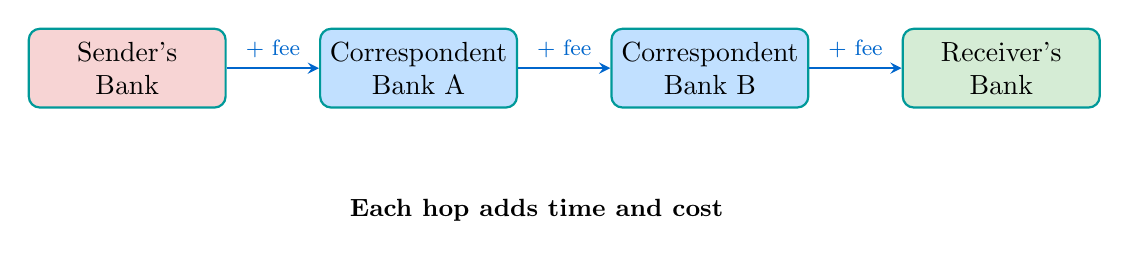
\begin{tikzpicture}[node distance=1.5cm]
% Traditional correspondent banking chain - NO dollar amounts
\node (sender) [blockchain, fill=dfred!20, align=center] {Sender's\\Bank};
\node (corr1) [blockchain, right of=sender, xshift=2.2cm, align=center] {Correspondent\\Bank A};
\node (corr2) [blockchain, right of=corr1, xshift=2.2cm, align=center] {Correspondent\\Bank B};
\node (receiver) [blockchain, right of=corr2, xshift=2.2cm, fill=dfgreen!20, align=center] {Receiver's\\Bank};

\draw[arrow] (sender) -- node[above, font=\footnotesize] {+ fee} (corr1);
\draw[arrow] (corr1) -- node[above, font=\footnotesize] {+ fee} (corr2);
\draw[arrow] (corr2) -- node[above, font=\footnotesize] {+ fee} (receiver);

% Label
\node[below of=corr1, xshift=1.5cm, yshift=-0.3cm, font=\small] {\textbf{Each hop adds time and cost}};
\end{tikzpicture}
\end{center}

\vspace{2mm}
\textbf{Why It Is Broken:}
\begin{itemize}\compactlist
\item Money must ``hop'' through several \textbf{correspondent banks}\footnotemark --- each one charges a fee and adds delay
\item Currency conversion happens at each hop, often at unfavorable rates
\item Compliance checks (anti-money laundering) at every intermediary slow the process further
\item The sender often does not know the total cost until the money arrives
\end{itemize}
\footnotetext{Correspondent banking --- a system where banks maintain accounts at other banks in foreign countries to facilitate international transfers.}
\end{frame}

% ---- Cross-Border Payments (cont.) ----
\begin{frame}{Cross-Border Payments: The Broken System (cont.)}
\begin{block}{The Insight}
Cross-border payments are the most expensive, slowest part of the payment system --- making them a prime target for FinTech disruption.
\end{block}
\end{frame}

% ==================== SLIDE 15: FINTECH SOLUTIONS FOR CROSS-BORDER ====================
\begin{frame}{FinTech Solutions for Cross-Border Payments}
\begin{alertblock}{The Problem}
How are companies trying to fix international payments?
\end{alertblock}

\vspace{1mm}
\begin{columns}[T]
\begin{column}{0.33\textwidth}
\begin{block}{Approach 1:\\Local Rail Matching}
\begin{itemize}\compactlist
\item Match senders and receivers in different countries
\item Use \textit{local} payment rails on each end
\item Money never actually crosses borders
\item Faster and cheaper than correspondent banking
\end{itemize}
\end{block}
\end{column}
\begin{column}{0.33\textwidth}
\begin{block}{Approach 2:\\Blockchain Settlement}
\begin{itemize}\compactlist
\item Use a shared digital ledger to transfer value
\item No correspondent banks needed
\item Settlement in minutes, not days
\item Requires adoption by both sides
\end{itemize}
\end{block}
\end{column}
\begin{column}{0.33\textwidth}
\begin{block}{Approach 3:\\Stablecoin Transfers}
\begin{itemize}\compactlist
\item Send digital tokens pegged to a currency
\item Available around the clock
\item Recipient converts to local currency
\item Regulatory status still evolving
\end{itemize}
\end{block}
\end{column}
\end{columns}

\vspace{1mm}
\begin{block}{The Insight}
Each approach trades off different dimensions: speed, cost, regulatory clarity, and adoption requirements. No single solution dominates yet --- the race to fix cross-border payments is still open.
\end{block}
\end{frame}

% ==================== SLIDE 16: WHEN PAYMENTS FAIL ====================
\begin{frame}{When Payments Fail}
\begin{alertblock}{The Problem}
What happens when a payment is declined --- and why does it matter more than you think?
\end{alertblock}

\vspace{2mm}
\begin{columns}[T]
\begin{column}{0.5\textwidth}
\textbf{Common Reasons Payments Fail:}
\begin{itemize}\compactlist
\item \textbf{Insufficient funds}: The most common cause
\item \textbf{Fraud blocks}: Automated systems flag suspicious activity
\item \textbf{Expired or invalid card}: Outdated payment credentials
\item \textbf{Network timeouts}: Technical failures between intermediaries
\item \textbf{Authentication abandonment}: Customer drops out during security checks
\end{itemize}

\vspace{2mm}
\textit{A \textbf{chargeback}\footnotemark\ is when a consumer disputes a transaction and the payment is reversed --- typically the merchant bears the cost.}
\footnotetext{Chargeback --- a consumer's right to dispute and reverse a card transaction within a defined window.}
\end{column}
\begin{column}{0.5\textwidth}
\begin{block}{The Hidden Cost of ``False Positives''}
A \textbf{false positive} occurs when a legitimate transaction is incorrectly blocked as fraud.

\vspace{2mm}
\textit{Why this matters:}
\begin{itemize}\compactlist
\item The customer may abandon the purchase entirely
\item The merchant loses revenue permanently
\item Customer trust and loyalty suffer
\item Blocking good transactions often costs \textbf{more} than the fraud it prevents
\end{itemize}
\end{block}
\end{column}
\end{columns}
\end{frame}

% ---- When Payments Fail (cont.) ----
\begin{frame}{When Payments Fail (cont.)}
\begin{exampleblock}{Think About It}
Has a legitimate purchase of yours ever been declined? How did it affect your experience?
\end{exampleblock}

\vspace{2mm}
\begin{block}{The Insight}
Payment optimization is not just about preventing fraud --- it is about finding the right balance between security and a smooth customer experience.
\end{block}
\end{frame}

% ==================== SLIDE 17: BUY NOW PAY LATER ====================
\begin{frame}{Buy Now Pay Later (BNPL)}
\begin{alertblock}{The Problem}
Why would a merchant pay \textit{higher} fees for installment payments?
\end{alertblock}

\vspace{2mm}
\begin{columns}[T]
\begin{column}{0.5\textwidth}
\textbf{How BNPL Works:}
\begin{enumerate}\compactlist
\item Consumer selects BNPL at checkout
\item BNPL provider pays the merchant (minus a fee)
\item Consumer repays in several installments
\item Typically no interest if payments are on time
\end{enumerate}

\vspace{2mm}
\textbf{Why Merchants Accept Higher Fees:}
\begin{itemize}\compactlist
\item Increases average order value
\item Attracts customers who might not buy otherwise
\item Converts browsers into buyers
\item Shifts credit risk to the BNPL provider
\end{itemize}
\end{column}
\begin{column}{0.5\textwidth}
\begin{block}{BNPL Revenue Sources}
\begin{itemize}\compactlist
\item \textbf{Merchant fees}: Higher than standard card fees --- the provider's main revenue
\item \textbf{Late payment fees}: Charged when consumers miss installments
\item \textbf{Interest}: On longer-term loan products
\end{itemize}
\end{block}
\end{column}
\end{columns}
\end{frame}

% ---- Buy Now Pay Later (cont.) ----
\begin{frame}{Buy Now Pay Later (BNPL) (cont.)}
\begin{alertblock}{Business Model Tensions}
\begin{itemize}
\item Credit losses without traditional underwriting\footnotemark
\item Growing regulatory scrutiny globally
\item Consumer debt accumulation concerns
\item Sustainability questions when growth slows
\end{itemize}
\end{alertblock}
\footnotetext{Underwriting --- the process of assessing whether a borrower is likely to repay.}

\vspace{2mm}
\begin{block}{The Insight}
BNPL shifts credit risk from consumers to providers, creating new business model tensions between growth and sustainability.
\end{block}
\end{frame}

% ==================== SLIDE 18: HANDS-ON NB02 ====================
\begin{frame}{Hands-On: NB02 Payment Transaction Analysis}
\begin{alertblock}{The Problem}
How do we analyze payment data to make better business decisions?
\end{alertblock}

\vspace{2mm}
\begin{block}{Notebook Overview}
Analyze simulated payment transaction data to understand:
\begin{itemize}\compactlist
\item How different payment methods compare in practice
\item How fee structures affect merchant profitability
\item How settlement times vary and why it matters for cash flow
\item How network analysis can reveal transaction patterns
\end{itemize}
\end{block}

\vspace{2mm}
\begin{columns}[T]
\begin{column}{0.5\textwidth}
\textbf{What You Will Do:}
\begin{itemize}\compactlist
\item Work with a realistic simulated payment dataset
\item Compare multiple payment methods across key dimensions
\item Visualize cost and settlement trade-offs
\item Build and analyze a payment network graph
\end{itemize}
\end{column}
\begin{column}{0.5\textwidth}
\begin{exampleblock}{No Programming Prerequisites}
The notebook is self-guided with code provided. Your job is to \textbf{interpret the results} and draw business conclusions --- not to write code from scratch.
\end{exampleblock}
\end{column}
\end{columns}
\end{frame}

% ---- Hands-On NB02 (cont.) ----
\begin{frame}{Hands-On: NB02 Payment Transaction Analysis (cont.)}
\begin{block}{The Insight}
Data analysis reveals patterns invisible in individual transactions --- what seems random at the single-payment level becomes predictable at scale.
\end{block}
\end{frame}

% ==================== SLIDE 19: NB02 EXERCISE TASKS ====================
\begin{frame}{NB02 Exercise Tasks}
\begin{columns}[T]
\begin{column}{0.5\textwidth}
\textbf{Part 1: Data Exploration}
\begin{itemize}
\item Load and examine the transaction dataset
\item Analyze how transaction amounts are distributed
\item Explore temporal patterns (e.g., business hours vs.\ weekends)
\item Calculate summary statistics by payment method
\end{itemize}

\vspace{3mm}
\textbf{Part 2: Fee Analysis}
\begin{itemize}
\item Compare fee structures across payment methods
\item Calculate effective fee rates at different transaction sizes
\item Determine which method is cheapest for different scenarios
\item Visualize cost curves to see where methods cross over
\end{itemize}
\end{column}
\begin{column}{0.5\textwidth}
\textbf{Part 3: Settlement Analysis}
\begin{itemize}
\item Examine how long different methods take to settle
\item Understand why the ``typical'' time can be misleading
\item Consider how settlement speed affects merchant cash flow
\end{itemize}

\vspace{3mm}
\textbf{Part 4: Network Analysis}
\begin{itemize}
\item Build a payment network graph from transaction data
\item Identify which parties are most connected (hubs)
\item Find critical bridges in the payment network
\item Analyze the direction of money flows
\end{itemize}

\vspace{3mm}
\begin{alertblock}{Key Skills Practiced}
Data exploration, visualization, comparative analysis, network thinking
\end{alertblock}
\end{column}
\end{columns}
\end{frame}

% ==================== SLIDE 20: DISCUSSION - PAYMENT CHOICE ====================
\begin{frame}{Discussion: Choosing Payment Methods}
\begin{block}{Scenario Analysis}
For each scenario, which payment method would you recommend and why? Think about the trade-offs.
\end{block}

\vspace{3mm}
\begin{columns}[T]
\begin{column}{0.5\textwidth}
\textbf{Scenario A: Monthly Rent Payment}
\begin{itemize}
\item Recurring, predictable amount
\item Speed is not critical
\item Minimizing cost matters most
\end{itemize}
\textcolor{dfgreen}{\textit{What method minimizes fees here?}}

\vspace{4mm}
\textbf{Scenario B: Small In-Store Purchase}
\begin{itemize}
\item Convenience and speed matter
\item High volume, low value per transaction
\item Customer experience is the priority
\end{itemize}
\textcolor{dfgreen}{\textit{What method optimizes for experience?}}
\end{column}
\begin{column}{0.5\textwidth}
\textbf{Scenario C: High-Value Property Transaction}
\begin{itemize}
\item Certainty of payment is essential
\item Large transfer amount
\item Legal requirements may apply
\end{itemize}
\textcolor{dfgreen}{\textit{What method provides maximum certainty?}}

\vspace{4mm}
\textbf{Scenario D: International Supplier Payment}
\begin{itemize}
\item Cross-border transfer needed
\item Currency conversion required
\item Balance of speed and cost
\end{itemize}
\textcolor{dfgreen}{\textit{Which newer approaches could help here?}}
\end{column}
\end{columns}

\vspace{3mm}
\textit{There are no single right answers --- the best method depends on the specific context and priorities.}
\end{frame}

% ==================== SLIDE 21: DISCUSSION - DISRUPTION ====================
\begin{frame}{Discussion: Where Will Disruption Happen?}
\begin{columns}[T]
\begin{column}{0.5\textwidth}
\textbf{Most Vulnerable to Disruption:}
\begin{itemize}
\item \textbf{Cross-border payments}: High friction, many intermediaries, strong incentive for alternatives
\item \textbf{Business-to-business payments}: Still heavily reliant on manual processes in many industries
\item \textbf{Interchange economics}: Regulatory pressure growing globally
\item \textbf{Settlement speed}: Real-time government infrastructure eroding the value of slow private rails
\end{itemize}
\end{column}
\begin{column}{0.5\textwidth}
\textbf{Most Protected from Disruption:}
\begin{itemize}
\item \textbf{Card networks}: Powerful network effects and deep merchant integration
\item \textbf{Settlement systems}: Government-operated, regulatory barriers to entry
\item \textbf{Consumer habits}: Trust, convenience, and inertia are powerful protectors
\end{itemize}

\vspace{3mm}
\begin{alertblock}{Discussion Questions}
\begin{enumerate}
\item If instant government payment rails are free, what happens to card networks?
\item Why haven't cryptocurrencies replaced traditional payments for everyday use?
\item What would it take to displace a dominant card network?
\end{enumerate}
\end{alertblock}
\end{column}
\end{columns}
\end{frame}

% ==================== SLIDE 22: EXECUTIVE SUMMARY ====================
\begin{frame}{Executive Summary: Key Takeaways}
\begin{enumerate}
\item \textbf{Payments are multi-layered}: Consumer interfaces $\rightarrow$ processors $\rightarrow$ networks $\rightarrow$ settlement systems. Each layer extracts value from every transaction.

\item \textbf{Speed vs.\ protection is the fundamental tradeoff}: Faster, cheaper payments are typically less reversible. Every payment method trades off these dimensions differently.

\item \textbf{Interchange funds the card ecosystem}: The issuing bank receives the largest share of fees because it bears credit and fraud risk. Merchants pass these costs to consumers through prices.

\item \textbf{Real-time government rails are reshaping competition}: When instant payments become free public infrastructure, the value shifts from moving money to the services built on top.

\item \textbf{Most FinTechs are layers, not replacements}: The majority of payment innovators build on top of existing rails rather than replacing them --- true disruption of the underlying infrastructure is rare.
\end{enumerate}

\vspace{3mm}
\begin{block}{One Sentence Summary}
Digital payments flow through a four-layer stack where each layer captures fees, and understanding this architecture reveals both where value is extracted and where FinTech disruption is possible.
\end{block}
\end{frame}

% ==================== SLIDE 23: CONCEPT MAP ====================
\begin{frame}{Concept Map: Digital Payments Ecosystem}
\begin{center}
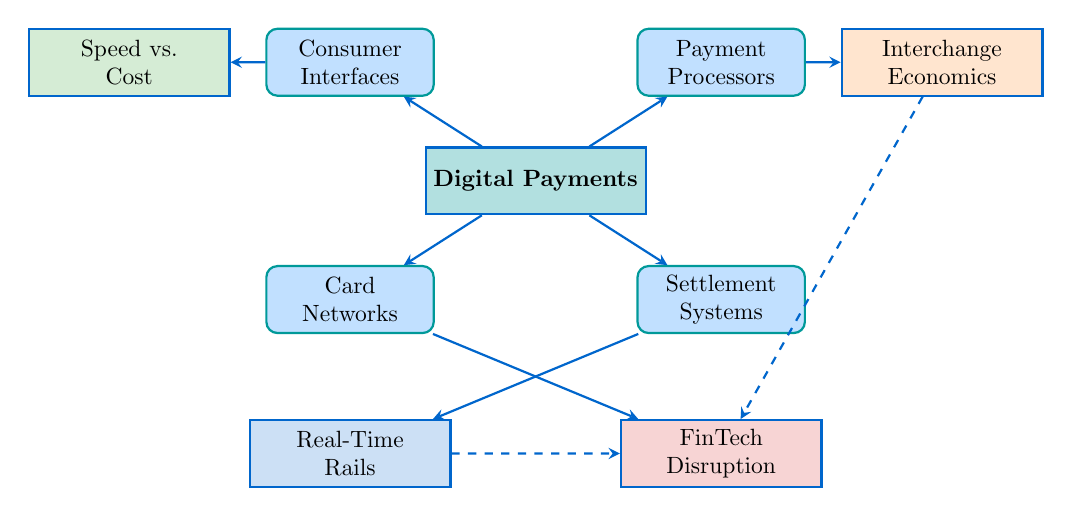
\begin{tikzpicture}[node distance=1.8cm, scale=0.85, transform shape]
% Central node
\node (payments) [process, fill=dfteal!30, minimum width=3cm] {\textbf{Digital Payments}};

% Layer nodes
\node (consumer) [blockchain, above left of=payments, xshift=-1.5cm, yshift=0.5cm, align=center] {Consumer\\Interfaces};
\node (processor) [blockchain, above right of=payments, xshift=1.5cm, yshift=0.5cm, align=center] {Payment\\Processors};
\node (network) [blockchain, below left of=payments, xshift=-1.5cm, yshift=-0.5cm, align=center] {Card\\Networks};
\node (settlement) [blockchain, below right of=payments, xshift=1.5cm, yshift=-0.5cm, align=center] {Settlement\\Systems};

% Concept nodes
\node (fee) [process, right of=processor, xshift=1.5cm, fill=dforange!20, align=center] {Interchange\\Economics};
\node (speed) [process, left of=consumer, xshift=-1.5cm, fill=dfgreen!20, align=center] {Speed vs.\\Cost};
\node (fintech) [process, below of=settlement, yshift=-0.5cm, fill=dfred!20, align=center] {FinTech\\Disruption};
\node (realtime) [process, below of=network, yshift=-0.5cm, fill=dfblue!20, align=center] {Real-Time\\Rails};

% Arrows
\draw[arrow] (payments) -- (consumer);
\draw[arrow] (payments) -- (processor);
\draw[arrow] (payments) -- (network);
\draw[arrow] (payments) -- (settlement);
\draw[arrow] (processor) -- (fee);
\draw[arrow] (consumer) -- (speed);
\draw[arrow] (settlement) -- (realtime);
\draw[arrow] (network) -- (fintech);
\draw[arrow, dashed] (realtime) -- (fintech);
\draw[arrow, dashed] (fee) -- (fintech);
\end{tikzpicture}
\end{center}

\vspace{2mm}
\textbf{Reading the map}: Each arrow shows a conceptual relationship. Dashed arrows indicate that real-time rails and interchange economics both drive FinTech disruption.
\end{frame}

% ==================== SLIDE 24: KEY TERMS ====================
\begin{frame}{Key Terms and Definitions}
\begin{description}
\item[\textcolor{dfblue}{Settlement}] The final, irrevocable transfer of funds from payer to payee. Distinct from authorization.

\item[\textcolor{dfblue}{Interchange}] The fee paid by the acquiring bank to the issuing bank for each card transaction. The issuing bank receives the largest share because it bears credit and fraud risk.

\item[\textcolor{dfblue}{Four-Party Model}] Card payment structure involving cardholder, merchant, issuing bank, and acquiring bank, connected by the card network.

\item[\textcolor{dfblue}{Float}] The time money is ``in transit'' between authorization and settlement, during which intermediaries may earn value on funds that have not yet moved.

\item[\textcolor{dfblue}{Chargeback}] A consumer's right to dispute and reverse a card transaction within a defined window. The merchant typically bears the cost.

\item[\textcolor{dfblue}{BNPL}] Buy Now Pay Later --- a payment method allowing consumers to split purchases into installments, typically with no interest if paid on time.

\item[\textcolor{dfblue}{Correspondent Banking}] A system where banks maintain accounts at other banks in foreign countries to facilitate international transfers --- each intermediary adds time and cost.
\end{description}
\end{frame}

% ==================== SLIDE 25: COMMON MISCONCEPTIONS ====================
\begin{frame}{Common Misconceptions}
\begin{columns}[T]
\begin{column}{0.5\textwidth}
\textbf{Myth 1:} ``Card payments are instant''\\
\textcolor{dfred}{Reality:} Authorization is instant, but settlement takes days. The merchant sees ``approved'' immediately, but does not receive the funds until later.

\vspace{5mm}
\textbf{Myth 2:} ``Wire transfers are always best for large amounts''\\
\textcolor{dfred}{Reality:} Wire transfers provide certainty, not cost efficiency. A simple bank transfer is often much cheaper --- wire transfers are chosen when guaranteed finality matters more than cost.
\end{column}
\begin{column}{0.5\textwidth}
\textbf{Myth 3:} ``FinTechs have replaced traditional payment rails''\\
\textcolor{dfred}{Reality:} Most payment FinTechs are layers \textit{on top of} existing infrastructure, not replacements. The underlying settlement systems remain largely the same.

\vspace{5mm}
\textbf{Myth 4:} ``Lower fees always mean a better payment method''\\
\textcolor{dfred}{Reality:} Speed, reversibility, and consumer protection all matter. The cheapest option may offer no recourse if something goes wrong --- sometimes paying more buys valuable protection.
\end{column}
\end{columns}
\end{frame}

% ==================== SLIDE 26: SELF-ASSESSMENT ====================
\begin{frame}{Self-Assessment}
\begin{block}{Question 1: The Payment Stack}
A new FinTech company builds a mobile payment app. Which layer of the payment stack are they primarily competing in, and why does this layer attract so much innovation?
\end{block}

\vspace{5mm}
\begin{block}{Question 2: Speed vs.\ Protection}
A consumer makes an instant, irrevocable payment and later discovers the product is defective. Why is this situation fundamentally different from a credit card purchase? What is the tradeoff?
\end{block}

\vspace{5mm}
\begin{block}{Question 3: Cross-Border Disruption}
Explain why cross-border payments are more expensive than domestic payments, and describe one FinTech approach that attempts to solve this problem.
\end{block}

\vspace{3mm}
\textit{If you can answer these three questions conceptually, you have mastered the key ideas of this topic.}
\end{frame}

% ==================== SLIDE 27: WHAT'S NEXT + QUESTIONS ====================
\begin{frame}{What's Next: Topic 2.2 --- The API Economy}
\begin{columns}[T]
\begin{column}{0.5\textwidth}
\textbf{Preview of T2.2:}
\begin{itemize}
\item How APIs enable non-banks to offer financial services
\item Open Banking: regulators requiring banks to share data
\item Banking-as-a-Service: renting banking infrastructure
\item Embedded finance: financial products inside non-financial apps
\end{itemize}

\vspace{3mm}
\textbf{Connection to Payments:}\\
APIs are how payment processors make integration simple for merchants --- the technology bridge between Layer 3 and the businesses that use it.
\end{column}
\begin{column}{0.5\textwidth}
\begin{block}{Key Question for T2.2}
How can a tech company offer you a bank account without being a bank?
\end{block}

\vspace{3mm}
\textbf{Hands-On: NB03}\\
Open Banking API Simulation --- make API calls to retrieve accounts, transactions, and initiate payments.

\vspace{5mm}
\begin{alertblock}{Action Item}
Complete \textbf{NB02 --- Payment Transaction Analysis} before starting Topic 2.2.
\end{alertblock}
\end{column}
\end{columns}

\vspace{3mm}
\centering
{\Large\textbf{Questions?}}

\bottomnote{Digital Finance -- Joerg Osterrieder}
\end{frame}

\end{document}
